% !TeX root = ../main.tex

\chapter{Fundamentals} \label{chapter:fundamentals}

To get a general understanding of how training a neural network works, we have to go through its theoretical concepts first. We start with the structure of simple feed-forward networks, continue with advanced model architectures that take advantage of the data's spatial or temporal properties, and finally end up with recent enhancements that we use throughout our final implementation.


\section{Neural Networks}

The main concept of neural networks (NN) dates back to the early 1950s, Warren McCulloch and Walter Pitts tried to build a mathematical model of information processing in our brain. Inspired by this work, Frank Rosenblatt developed the so called \textit{perceptron} about two decades later \parencite[p. 226]{pattern_and_ml}. The perceptron itself is has quite a simple structure. It is usually visualized as a node that consists any number of binary inputs $ x_{i} $, as well as a single output $ y_{out} $ with $ x_{i}, y_{out} \in \{0, 1\} $. In addition, each input is weighted by $ w_{i} \in \rm I\!R $ to express importance of each particular input. The output is determined by the simple rule that the weighted sum of all inputs has to reach a specified threshold to make the perceptron fire its output \parencite{neural_nets_deep_learning}. Usually, this threshold is usually called bias $ b \in \rm I\!R $, defined as the negative threshold. All of this can be expressed as follows:

\begin{equation} \label{eq:mlp}
  y_{out} = \begin{cases}
    1, & \text{if $ \sum\limits_{i=1}^n \, w_{i}x_{i} + b > 0$}.\\
    0, & \text{otherwise}.
  \end{cases}
\end{equation}

Even that its formulation is that simple, it can represent complex decision-making when we stack multiple elements togther, known as multilayer perceptrons (MLP). Such a network is illustrated in figure \ref{fig:mlp}.

\begin{figure}[htpb]
	\centering
	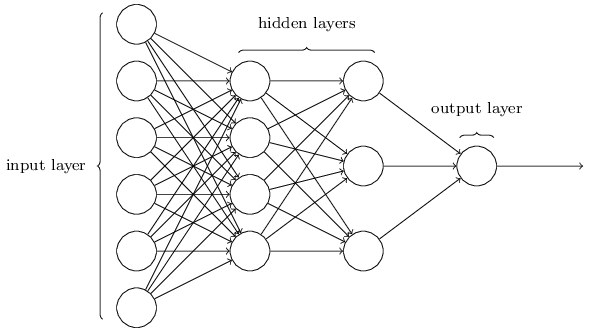
\includegraphics[scale=0.35]{figures/mlp.png} % TODO: highlight perceptron in BOLD
	\caption{Example of a MLP. A single perceptron is highlighted in bold.} \label{fig:mlp}
\end{figure}

The first and last layer of such a network are refered as \textit{input layer} and \textit{output layer} and their number is determined by the given problem to solve. In case we want to train a network that identifies human faces in colored pictures with height and width of 100 pixels, it would require our input layer to have $ n_{input}=3000 $ perceptrons, as well as a single output. In contrary, all intermediate layers are known as \textit{hidden layers} and can have any number of elements and depth. Afterwards, we can feed the input layer with a data example and apply equation \ref{eq:mlp} in each node to retrieve our binary result. This prediction step is called \textit{inference}. But in order to retrive meaningful results, we have to train our network first.

\subsection{Network Training}

The final goal of training such a network is to end up with a model that generalizes on any kind of data from the same class \parencite[p. 2]{pattern_and_ml}. The data that is used during this process is called \textit{training set}, the data that evaluates its generalization capabilites \textit{test set}. Since we know the ground truth outcome of this data example during the training phase, we can quantify the outcome using a loss function\footnote{Also known as cost function, objective function or error function. We use the averaged variants for all presented functions, because therefore we achieve pixel-wise results that are independent regarding the image dimensions later on when performing frame prediction. Additionally, the non-averaged versions of MAE and MSE are known as $ \ell_{1} $ and $ \ell_{2} $.}, such as \textit{mean absolute error} (MAE):

\begin{equation} \label{eq:mae}
  \mathcal{L}_{MAE}(w, b)=\frac{1}{N} \sum\limits_{x} | y_{out}(x) - t |
\end{equation}

\textit{mean squared error} (MSE):

\begin{equation} \label{eq:mse}
  \mathcal{L}_{MSE}(w, b)=\frac{1}{N} \sum\limits_{x} \| y_{out}(x) - t \|^2
\end{equation}

or \textit{binary cross-entropy} (BCE) \parencite{conv_lstm_nowcasting}:

\begin{equation} \label{eq:bce}
  \mathcal{L}_{BCE}(w, b)= -\frac{1}{N} \sum\limits_{x} t \log{y_{out}(x)} + (1-t) \log{(1-y_{out}(x))} 
\end{equation}

where $ N $ is the number of outcomes and $ t $ the ground truth target. Many other functions exist, but these are the main objectives that we use in later chapters. During training our network, we want to find the set of weights $ w $ and biases $ b $ that minimizes our error:

\begin{equation} \label{eq:min-loss}
  arg\min_x \mathcal{L}(w, b)
\end{equation}

At this point, we face the fundamental problem of perceptrons. Because in order find the best set of parameters, we have to do small changes in $ w $ and $ b $ to justify the output into the right direction of the desired outcome. But since the perceptron's output is binary, a small change can cause a sudden flip in the overall output. To overcome this issue, we replace these perceptrons with \textit{neurons}:

\begin{equation}
\begin{aligned}
z &= \sum\limits_{i=1}^n \, w_{i}x_{i} + b \\
y_{out} &= a(z)
\end{aligned}
\end{equation}

which allow $ x_{i}, y_{out} \in \rm I\!R $ using an \textit{activation function} $ a(z) $. Frequently used examples are the sigmoid function $ \sigma(z) $, hyperbolic tangent $ tanh(z) $ and the rectified linear unit (ReLu) $ max(0, z) $. These are displayed in figure \ref{fig:activations}.

\begin{figure}[htpb]
  \centering
  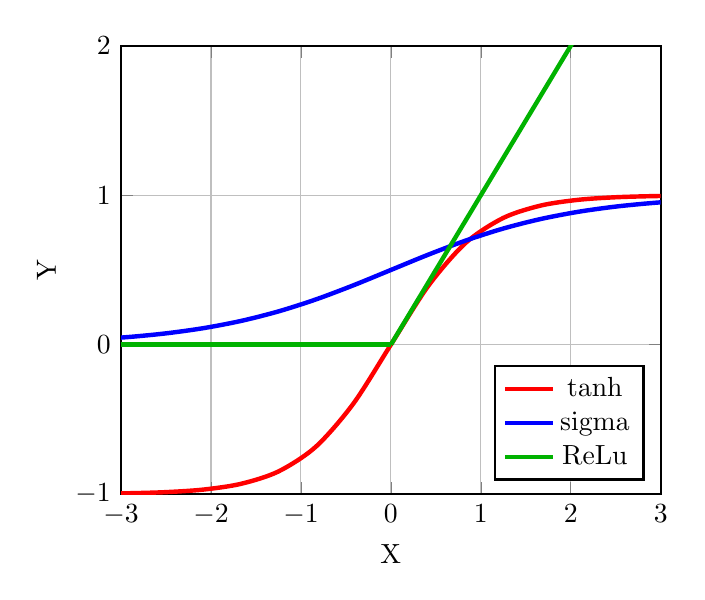
\begin{tikzpicture}
    \begin{axis}[
        ymin=-1,
        ymax=2,
        xmin=-3,
        xmax=3,
        legend style={legend pos=south east},
        grid,
        thick,
        ylabel=Y,
        xlabel=X
      ]
      \addplot [mark=none,draw=red,smooth,ultra thick] {tanh(\x)};
      \addlegendentry{tanh};
      \addplot [mark=none,draw=blue,smooth,ultra  thick] {1/(1+exp(-1*(\x))};
      \addlegendentry{sigma};
      \addplot[mark=none,draw=black!30!green,ultra thick,smooth,domain=0:3] {x};
	  \addplot[mark=none,draw=black!30!green,ultra thick,smooth,domain=-3:0] {0};
      \addlegendentry{ReLu};
    \end{axis}
  \end{tikzpicture}
  \caption[Activation functions]{Diagrams of the most frequently used activation function in neural networks.}\label{fig:activations}
\end{figure}

# TODO: continue here?

2. how to init the weights and bias in first place? --> random --> mention xavier and its formular
3. how how do we find the min params? --> grad descent?
(Back to our example of face detection, we would ... ?)

\subsubsection{Regularization}

\subsubsection{Gradiend Descent}

Explain GD, why SGD is used. And also introduce Adam here already?

\subsubsection{Hyperparameter}

















\section{Convolutional Neural Networks}

Networks for spatial learning...

\subsubsection{History}
Short history as intro LeCun, OCR, ...

\subsection{Benefits}

(1) Param sharing, (2) sparsity, (3) ...

\subsection{Convolutional Operation}

Explain the conv op

\subsection{Transposed Convolutional Operation}

What is the conv-t op. Foot comment: Should not be called deconv

\subsection{Fully-convolutional Networks}

What are FCNs and what is their benefit?


\section{Recurrent Neural Networks}

Networks for temporal learning...

\subsection{RNN}

Bla bla...

\subsubsection{History}
Short intro (history) to RNNs

\subsubsection{Architecture}
explain it in with a small diagram

\subsubsection{BPTT}
What is BPTT in comparision to back propagation

\subsubsection{Drawbacks}
What are the drawbacks of RNNs: vanishing/explosion of gradients problem

\subsection{LSTM}

Bla bla

\subsubsection{History}
Short intro (history) to LSTMs (Hochreiter, Schmidhuber)

\subsubsection{Architecture}
Show differences to classical RNNs

\subsubsection{Benefits}
How does this suspensate the drawbacks of RNNs (gates, ...)


\section{Autoencoder Networks}

What are autoencoder networks?


\section{Parameter initialization}

Explain why they are randomly initialized. Why xavier method? How is xavier-init defined?


\section{Batch Normalization}


\section{Perceptuall Similarity of Images}

Introduce perceptual similarity and explain some metrics (SSIM, PSNR, GDL?) which we will use in evaluation.
Why is perceptuall loss so important? Example of chess/zebra image?

